% =============================================================================
%  QED-CIS in the cqed-scf package: formalism, working equations, and algorithms
%
%  Overleaf-ready: a single self-contained file, no external .bib required.
%  To use BibTeX instead, delete the thebibliography environment at the end and
%  point \bibliography at your own file.
%
%  Companion documents:
%    docs/development/QED_RESPONSE_PLAN.md   -- implementation plan and status
%    docs/development/psi4_array_aliasing.md -- a defect note referenced in Sec. 9
% =============================================================================
\documentclass[11pt]{article}

\usepackage[margin=1in]{geometry}
\usepackage{amsmath, amssymb, mathtools, bm}
\usepackage{booktabs}
\usepackage{braket}
\usepackage{tikz}
\usepackage{algorithm}
\usepackage{algpseudocode}
\usepackage{enumitem}
\usepackage{microtype}
\usepackage[dvipsnames]{xcolor}
\usepackage[colorlinks=true, linkcolor=BrickRed, citecolor=BrickRed,
            urlcolor=NavyBlue]{hyperref}

% ---- macros ----------------------------------------------------------------
\newcommand{\lam}{\bm{\lambda}}
\newcommand{\dop}{\hat{d}}                      % lambda . mu_el (one-electron)
\newcommand{\dexp}{\langle d \rangle}
\newcommand{\Hpf}{\hat{H}_{\mathrm{PF}}}
\newcommand{\Ecqed}{E_{\mathrm{CQED\text{-}SCF}}}
\newcommand{\nph}{N_{\mathrm{ph}}}
\newcommand{\nov}{n_{ov}}
\newcommand{\nocc}{n_{o}}
\newcommand{\nvir}{n_{v}}
\newcommand{\bd}{\hat{b}^{\dagger}}
\newcommand{\bo}{\hat{b}}
\DeclareMathOperator{\Tr}{Tr}

\title{\textbf{QED-CIS in \texttt{cqed-scf}}\\[2pt]
\large Formalism, working equations, and the matrix-free algorithm}
\author{}
\date{}

\begin{document}
\maketitle
\vspace{-3em}

\begin{abstract}
\noindent
This note documents the cavity QED configuration-interaction-singles (QED-CIS)
implementation in the \texttt{cqed-scf} package. It fixes the Pauli--Fierz
Hamiltonian and coherent-state convention, defines the composite
electron--photon basis and the index ordering used internally, gives every
matrix-element block explicitly, and specifies the matrix-free
$\bm{\sigma}$-build and iterative eigensolver that replace the explicit
Hamiltonian construction. Sections marked \emph{implementation note} record
choices specific to this code that a reader comparing against the literature
would otherwise find surprising --- in particular the analytic cancellation of
two terms that appear explicitly in most published formulations
(Sec.~\ref{sec:cancellation}), and the fact that the eigenvalues are referenced
to the CQED-SCF energy rather than to the correlated ground state
(Sec.~\ref{sec:zero}).
\end{abstract}

\tableofcontents
\bigskip

% =============================================================================
\section{Scope and notation}

The implementation targets \emph{Hermitian} QED-CIS with a real cavity frequency.
The non-Hermitian, lossy-cavity generalisation of Ref.~\cite{McTague2022}
is deliberately out of scope; the solver interface is left open to it but no
complex-$\omega$ path is implemented.

\begin{table}[h]
\centering
\small
\begin{tabular}{@{}ll@{}}
\toprule
symbol & meaning \\
\midrule
$i,j,k$ / $a,b,c$ / $p,q,r,s$ & occupied / virtual / general molecular orbitals \\
$\nocc, \nvir$, $\nov=\nocc\nvir$ & counts of occupied, virtual, and singly-excited configurations \\
$n,m$ & photon-number (Fock) indices, $0 \le n \le \nph$ \\
$\lam$ & cavity coupling vector, $\lam = \sqrt{1/\epsilon_0 V}\,\hat{\bm{e}}$ \\
$\omega$ & cavity mode frequency (real) \\
$\hat{\bm{\mu}}$ & total dipole operator; $\hat{\bm{\mu}}_{\mathrm{el}}$ its electronic part \\
$\dop$ & $\lam\cdot\hat{\bm{\mu}}_{\mathrm{el}}$, a one-electron operator; $d_{pq}$ its MO matrix elements \\
$\dexp$ & $\lam\cdot\langle\hat{\bm{\mu}}_{\mathrm{el}}\rangle$ over the CQED-SCF reference \\
$\bd, \bo$ & photon creation / annihilation operators \\
$\ket{\Phi_0}$ & CQED-SCF (or canonical HF) reference determinant \\
$\ket{\Phi_i^a}$ & singlet spin-adapted single excitation \\
$F_{pq}$ & Pauli--Fierz Fock matrix in the chosen MO basis \\
$(pq|rs)$ & two-electron repulsion integrals, chemists' notation \\
$g$ & $\sqrt{\omega/2}$ \\
\bottomrule
\end{tabular}
\caption{Notation used throughout.}
\end{table}

Only closed-shell, singlet-adapted excitations are treated. Triplets decouple
from the bilinear light--matter term (their transition dipole
$\braket{\Phi_0 | \dop | {}^3\Phi_i^a}$ vanishes) but \emph{not} from the
$\bm{G}$ block of Sec.~\ref{sec:G}; they are not implemented.

% =============================================================================
\section{The Pauli--Fierz Hamiltonian and the coherent-state basis}

In the dipole (long-wavelength) approximation and length gauge, a single cavity
mode coupled to a molecule is described by the Pauli--Fierz
Hamiltonian~\cite{Haugland2020, DePrince2021}
\begin{equation}
\Hpf
= \hat{H}_{\mathrm{el}}
\;+\; \omega\,\bd\bo
\;-\; \sqrt{\tfrac{\omega}{2}}\,
      \bigl(\lam\cdot\hat{\bm{\mu}}\bigr)\bigl(\bd + \bo\bigr)
\;+\; \tfrac{1}{2}\bigl(\lam\cdot\hat{\bm{\mu}}\bigr)^{2},
\label{eq:PF}
\end{equation}
where $\hat{H}_{\mathrm{el}}$ is the usual electronic Hamiltonian, the third
term is the bilinear light--matter coupling, and the fourth is the dipole
self-energy (DSE).

\subsection{Coherent-state transformation}

Working directly in the photon-number basis makes the reference determinant
couple to the one-photon state, because
$\braket{\Phi_0 | \lam\cdot\hat{\bm{\mu}} | \Phi_0} \ne 0$. Applying the
coherent-state displacement operator that removes the reference expectation
value~\cite{Haugland2020, McTague2022} replaces
$\lam\cdot\hat{\bm{\mu}} \to \lam\cdot\hat{\bm{\mu}} - \langle \lam\cdot\hat{\bm{\mu}}\rangle$
in both the bilinear and DSE terms:
\begin{equation}
\Hpf^{\mathrm{CS}}
= \hat{H}_{\mathrm{el}}
+ \omega\,\bd\bo
- \sqrt{\tfrac{\omega}{2}}\,\Delta\hat{d}\,(\bd + \bo)
+ \tfrac{1}{2}\bigl(\Delta\hat{d}\bigr)^{2},
\qquad
\Delta\hat{d} \equiv \lam\cdot\hat{\bm{\mu}} - \langle\lam\cdot\hat{\bm{\mu}}\rangle .
\label{eq:PFCS}
\end{equation}
This is the form used throughout. Its immediate consequence, used repeatedly
below, is
\begin{equation}
\braket{\Phi_0, n | \Hpf^{\mathrm{CS}} | \Phi_0, n\pm1} = 0 ,
\label{eq:refref}
\end{equation}
i.e.\ the reference determinant does not couple to its own photon replicas.

\subsection{One- and two-electron decomposition of the DSE}
\label{sec:dsedecomp}

Write $\dop = \lam\cdot\hat{\bm{\mu}}_{\mathrm{el}}$. Squaring the electronic
dipole separates into a one-electron and a two-electron piece,
\begin{equation}
\tfrac{1}{2}\Bigl(\sum_i \dop(i)\Bigr)^{2}
= \underbrace{\tfrac{1}{2}\sum_i \dop(i)^2}_{\text{one-electron}}
+ \underbrace{\tfrac{1}{2}\sum_{i \ne j} \dop(i)\,\dop(j)}_{\text{two-electron}} .
\label{eq:dsesplit}
\end{equation}
The one-electron piece is quadrupolar: with $\dop = \lam\cdot\bm{r}$ up to sign
conventions, $\dop^2$ contracts the Cartesian quadrupole integrals against
$\lambda_x\lambda_y$. In the code this is
\begin{equation}
Q^{\mathrm{PF}}_{\mu\nu} =
-\tfrac{1}{2}\sum_{xy} \lambda_x \lambda_y \, Q^{xy}_{\mu\nu},
\label{eq:QPF}
\end{equation}
added to the core Hamiltonian, $\bm{H} = \bm{H}_0 + \bm{Q}^{\mathrm{PF}}$.

\paragraph{The two-electron DSE is an ERI with a separable kernel.}
This is the single most useful structural observation in this document. The
operator $\dop(1)\dop(2)$ has exactly the form of a two-electron repulsion
operator with the rank-one kernel
\begin{equation}
(pq|rs) \;\longrightarrow\; d_{pq}\, d_{rs} .
\label{eq:sepkernel}
\end{equation}
Every Slater--Condon result for the ERIs therefore carries over verbatim with
that substitution --- which is where the DSE block $\bm{\Delta}$ of
Sec.~\ref{sec:Delta} comes from, and why it costs $O(N^3)$ rather than
requiring any four-index quantity (Sec.~\ref{sec:sigma}).

\subsection{The CQED-SCF reference}

The reference determinant is obtained from a self-consistent solution of the
Pauli--Fierz mean-field equations, giving the Fock matrix
\begin{equation}
F_{\mu\nu} = H^0_{\mu\nu} + Q^{\mathrm{PF}}_{\mu\nu}
 + 2J_{\mu\nu}[D] - K_{\mu\nu}[D] - N_{\mu\nu}[D],
\qquad
N_{\mu\nu}[D] = \sum_{\rho\sigma} d_{\mu\rho}\, d_{\nu\sigma} D_{\rho\sigma},
\label{eq:fock}
\end{equation}
with $\bm{D}$ the closed-shell density. Orbitals may alternatively be taken from
a cavity-free canonical HF calculation; see Sec.~\ref{sec:orbitals}.

\subsection{Implementation note: two terms that cancel analytically}
\label{sec:cancellation}

Most published formulations of the coherent-state CQED-RHF Fock operator carry
two additional terms that are absent from Eq.~\eqref{eq:fock}: a mean-field DSE
contribution $\bm{M}$ and a one-electron coherent-state shift $\bm{d}^{\mathrm{PF}}$,
\begin{equation}
M_{\mu\nu} = d_{\mu\nu} \Tr(\bm{d}\bm{D}), \qquad
d^{\mathrm{PF}}_{\mu\nu}
 = \bigl(\lam\cdot\bm{\mu}_{\mathrm{nuc}} - \lam\cdot\langle\bm{\mu}\rangle\bigr) d_{\mu\nu}.
\end{equation}
Writing $x \equiv \lam\cdot\langle\bm{\mu}_{\mathrm{el}}\rangle = 2\Tr(\bm{d}\bm{D})$
and $n_{\mathrm{nuc}} \equiv \lam\cdot\bm{\mu}_{\mathrm{nuc}}$, these are
$2\bm{M} = x\,\bm{d}$ and
$\bm{d}^{\mathrm{PF}} = (n_{\mathrm{nuc}} - x - n_{\mathrm{nuc}})\bm{d} = -x\,\bm{d}$, so
\begin{equation}
\boxed{\; 2\bm{M} + \bm{d}^{\mathrm{PF}} = \bm{0} \;}
\label{eq:fockcancel}
\end{equation}
identically. The corresponding energy contributions cancel against the DSE
constant $d_c$:
\begin{equation}
\Tr\bigl[2\bm{M}\bm{D}\bigr] = +\tfrac{1}{2}x^2, \quad
\Tr\bigl[2\bm{d}^{\mathrm{PF}}\bm{D}\bigr] = -x^2, \quad
d_c = \tfrac{1}{2}n_{\mathrm{nuc}}^2 - n_{\mathrm{nuc}}(x + n_{\mathrm{nuc}}) + \tfrac{1}{2}(x+n_{\mathrm{nuc}})^2 = +\tfrac{1}{2}x^2,
\label{eq:encancel}
\end{equation}
whose sum vanishes. The implementation therefore omits all three, which makes
its Fock matrix and total energy \emph{identical} --- not merely equivalent --- to
formulations that carry them. Both identities are asserted numerically in the
test suite, so the simplification cannot silently rot.

% =============================================================================
\section{The QED-CIS ansatz and basis ordering}
\label{sec:basis}

\subsection{Basis}

The composite electron--photon basis is
\begin{equation}
\Bigl\{\;\ket{\Phi_0} \otimes \ket{n},\;\;
        \ket{\Phi_i^a} \otimes \ket{n} \;\Bigr\},
\qquad n = 0,\dots,\nph ,
\end{equation}
of dimension $(\nph+1)(1+\nov)$. Setting $\nph = 1$ recovers the QED-CIS-1
method of Ref.~\cite{McTague2022}; the implementation is general in $\nph$
at no additional cost (Sec.~\ref{sec:blocks}).

\subsection{Index ordering}

Configurations are ordered \emph{photon-major}, with the reference determinant
leading each photon block:
\begin{equation}
\boxed{\;
\mathrm{index}(n,p) = n\,(1 + \nov) + p,
\qquad
p =
\begin{cases}
0, & \ket{\Phi_0, n} \\[2pt]
1 + i\,\nvir + a, & \ket{\Phi_i^a, n}
\end{cases}
\;}
\label{eq:index}
\end{equation}

\paragraph{Why not photon-minor.} An interleaved ordering such as
$\mathrm{index} = 2(i\,\nvir + a) + n + 2$, used in earlier reference
implementations, scatters the electronic block --- which is \emph{identical} in
every photon sector --- across alternating rows and columns. It cannot be
sliced, cannot be reused between photon sectors, forces an explicit six-deep
loop over $(i,a,n,j,b,m)$ to construct, and hard-codes two Fock states. The two
orderings are related by a permutation and have identical spectra; only one of
them exposes structure a $\bm{\sigma}$ routine can exploit.

\subsection{Block structure}
\label{sec:blocks}

In the ordering of Eq.~\eqref{eq:index} the Hamiltonian is block-tridiagonal in
photon number, built from just \emph{two} photon-independent blocks:

\begin{center}
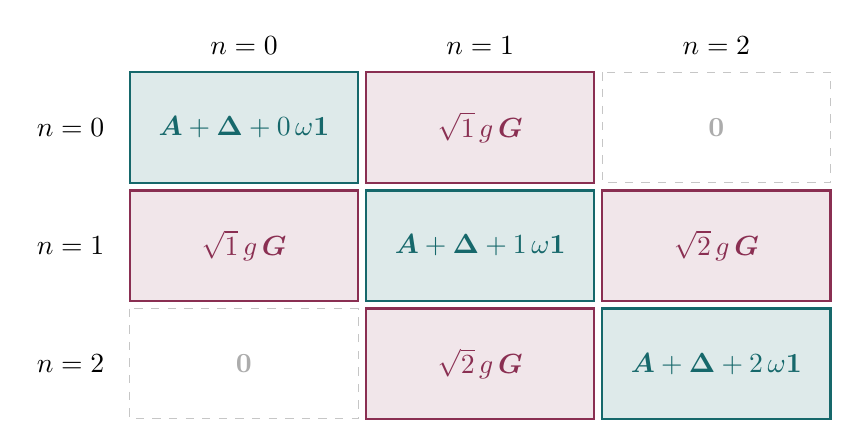
\begin{tikzpicture}[scale=1.0]
  \definecolor{elec}{RGB}{22,104,107}
  \definecolor{coup}{RGB}{138,47,82}
  \foreach \rowi in {0,1,2} {
    \foreach \colj in {0,1,2} {
      \pgfmathtruncatemacro{\dist}{abs(\rowi-\colj)}
      \pgfmathtruncatemacro{\rung}{max(\rowi,\colj)}
      \ifnum\dist=0
        \fill[elec!14] (\colj*3.0, -\rowi*1.5) rectangle ++(2.9, -1.4);
        \draw[elec, thick] (\colj*3.0, -\rowi*1.5) rectangle ++(2.9, -1.4);
        \node[elec] at (\colj*3.0+1.45, -\rowi*1.5-0.7)
             {$\bm{A}+\bm{\Delta}+\rowi\,\omega\bm{1}$};
      \else
        \ifnum\dist=1
          \fill[coup!12] (\colj*3.0, -\rowi*1.5) rectangle ++(2.9, -1.4);
          \draw[coup, thick] (\colj*3.0, -\rowi*1.5) rectangle ++(2.9, -1.4);
          \node[coup] at (\colj*3.0+1.45, -\rowi*1.5-0.7) {$\sqrt{\rung}\,g\,\bm{G}$};
        \else
          \draw[gray!45, dashed] (\colj*3.0, -\rowi*1.5) rectangle ++(2.9, -1.4);
          \node[gray!65] at (\colj*3.0+1.45, -\rowi*1.5-0.7) {$\bm{0}$};
        \fi
      \fi
    }
  }
  \foreach \kk in {0,1,2} {
    \node[anchor=east] at (-0.2, -\kk*1.5-0.7) {$n=\kk$};
    \node[anchor=south] at (\kk*3.0+1.45, 0.1) {$n=\kk$};
  }
\end{tikzpicture}
\end{center}

\noindent
Only $\bm{A}+\bm{\Delta}$ and $\bm{G}$ are ever constructed; the $\sqrt{n+1}$
factors are scalars. Consequently \textbf{QED-CIS-$N$ requires no additional
code beyond QED-CIS-1}. Putting the reference determinant first within each
block keeps the electronic sub-block a contiguous $\nov \times \nov$ slice,
which can be compared directly against ordinary CIS.

% =============================================================================
\section{Matrix elements}

All energies below are referenced to $\Ecqed$ (see Sec.~\ref{sec:zero}).

\subsection{Photon block \texorpdfstring{$\bm{\Omega}$}{Omega}}

The bare photon term $\omega\bd\bo$ is diagonal:
\begin{equation}
\braket{\Phi_0, n | \omega\bd\bo | \Phi_0, m} = n\omega\,\delta_{nm},
\qquad
\braket{\Phi_i^a, n | \omega\bd\bo | \Phi_j^b, m}
 = n\omega\,\delta_{nm}\delta_{ij}\delta_{ab}.
\end{equation}
It contributes $n\omega\bm{1}$ to the $n$-th diagonal block.

\subsection{Electronic block \texorpdfstring{$\bm{A}$}{A}}

With a general (not necessarily canonical) Pauli--Fierz Fock matrix,
\begin{equation}
\boxed{\;
A_{ia,jb}
= \underbrace{\delta_{ij}F_{ab} - \delta_{ab}F_{ij}}_{\text{one-electron}}
\;+\; \underbrace{2(ia|jb) - (ij|ab)}_{\text{two-electron}}
\;}
\label{eq:A}
\end{equation}
and the reference--singles coupling within a photon sector is the Brillouin
element
\begin{equation}
\braket{\Phi_0, n | \hat{H} | \Phi_i^a, n} = \sqrt{2}\,F_{ia}.
\label{eq:brillouin}
\end{equation}
For canonical CQED-SCF orbitals $F_{ij} = \delta_{ij}\varepsilon_i$,
$F_{ab} = \delta_{ab}\varepsilon_a$ and $F_{ia} = 0$, so Eq.~\eqref{eq:A}
collapses to the familiar
$\delta_{ij}\delta_{ab}(\varepsilon_a - \varepsilon_i) + 2(ia|jb) - (ij|ab)$
and Eq.~\eqref{eq:brillouin} vanishes.

\subsection{Dipole self-energy block \texorpdfstring{$\bm{\Delta}$}{Delta}}
\label{sec:Delta}

The one-electron DSE contributions of Sec.~\ref{sec:dsedecomp} are already
inside $\bm{F}$: the quadrupole term $\bm{Q}^{\mathrm{PF}}$ sits in the core
Hamiltonian and the mean-field DSE enters through $-\bm{N}[\bm{D}]$ in
Eq.~\eqref{eq:fock}, while the coherent-state one-electron shift cancels
identically (Sec.~\ref{sec:cancellation}). What remains explicitly in the CIS
matrix is the two-electron DSE, obtained from
$2(ia|jb) - (ij|ab)$ under the separable substitution~\eqref{eq:sepkernel}:
\begin{equation}
\boxed{\;
\Delta_{ia,jb}
= \underbrace{2\,d_{ia}\,d_{jb}}_{\text{``Coulomb-like''}}
\;-\; \underbrace{d_{ij}\,d_{ab}}_{\text{``exchange-like''}}
\;}
\label{eq:Delta}
\end{equation}
The first term is rank one in the composite index $(ia)$; the second is
separable into $\nocc\times\nocc$ and $\nvir\times\nvir$ factors. Neither
requires a four-index object, which is what makes the DSE essentially free in
the $\bm{\sigma}$ build.

\subsection{Bilinear coupling block \texorpdfstring{$\bm{G}$}{G}}
\label{sec:G}

The coupling operator is
$-g\,\Delta\hat{d}\,(\bd+\bo)$ with $g = \sqrt{\omega/2}$. Its electronic part
is one-electron, so between singles
\begin{equation}
\boxed{\;
G_{ia,jb} = \delta_{ab}\,d_{ij} - \delta_{ij}\,d_{ab}
\;}
\label{eq:G}
\end{equation}
and between the reference and a single,
$\braket{\Phi_0 | (-\Delta\hat{d}) | \Phi_i^a} = -\sqrt{2}\,d_{ia}$. Combining
with the photon ladder matrix elements
$\braket{n\pm1|(\bd+\bo)|n} = \sqrt{n+1}$ or $\sqrt{n}$ gives
\begin{align}
\braket{\Phi_i^a, n\!+\!1 | \hat{H} | \Phi_j^b, n}
 &= \sqrt{n+1}\;g\;G_{ia,jb},
\label{eq:Gss}\\[2pt]
\braket{\Phi_0, n\!+\!1 | \hat{H} | \Phi_i^a, n}
 = \braket{\Phi_0, n | \hat{H} | \Phi_i^a, n\!+\!1}
 &= -\sqrt{(n+1)\,\omega}\;d_{ia},
\label{eq:Grs}
\end{align}
the latter using $\sqrt{2}\,g = \sqrt{\omega/2}\cdot\sqrt{2} = \sqrt{\omega}$.
Note $\bm{G}$ is symmetric, and by Eq.~\eqref{eq:refref} there is no
reference--reference coupling across photon sectors.

\subsection{Summary}

\begin{table}[h]
\centering
\small
\renewcommand{\arraystretch}{1.35}
\begin{tabular}{@{}lll@{}}
\toprule
block & element & note \\
\midrule
$\braket{\Phi_0,n|\hat{H}|\Phi_0,n}$ & $n\omega$ & photon ladder \\
$\braket{\Phi_0,n|\hat{H}|\Phi_0,n\pm1}$ & $0$ & coherent-state basis, Eq.~\eqref{eq:refref} \\
$\braket{\Phi_0,n|\hat{H}|\Phi_i^a,n}$ & $\sqrt{2}\,F_{ia}$ & zero only for canonical CQED orbitals \\
$\braket{\Phi_i^a,n|\hat{H}|\Phi_j^b,n}$ & $A_{ia,jb} + \Delta_{ia,jb} + n\omega\,\delta_{ij}\delta_{ab}$ & Eqs.~\eqref{eq:A}, \eqref{eq:Delta} \\
$\braket{\Phi_0,n\!+\!1|\hat{H}|\Phi_i^a,n}$ & $-\sqrt{(n\!+\!1)\omega}\;d_{ia}$ & Eq.~\eqref{eq:Grs} \\
$\braket{\Phi_i^a,n\!+\!1|\hat{H}|\Phi_j^b,n}$ & $\sqrt{n\!+\!1}\;g\;G_{ia,jb}$ & Eq.~\eqref{eq:Gss} \\
\bottomrule
\end{tabular}
\caption{Complete set of QED-CIS matrix elements in the basis of
Sec.~\ref{sec:basis}. All other blocks vanish.}
\label{tab:elements}
\end{table}

% =============================================================================
\section{Orbital basis: canonical HF versus CQED-SCF}
\label{sec:orbitals}

Because Eq.~\eqref{eq:A} is written with a general $\bm{F}$, either orbital set
may be used. They are \emph{not} equivalent, and the difference is physical
rather than an error:

\begin{itemize}[leftmargin=1.4em, itemsep=3pt]
\item \textbf{Electronic non-invariance.} CIS is invariant under separate
occupied--occupied and virtual--virtual rotations, but \emph{not} under
occupied--virtual rotations. Canonical HF and CQED-SCF orbitals differ by
exactly such a rotation --- that rotation \emph{is} the cavity-induced orbital
relaxation --- so $\{\ket{\Phi_0}\} \cup \{\ket{\Phi_i^a}\}$ spans a different
space in each basis. This never vanishes for CIS; it would vanish for FCI, or
for CAS within its active space.
\item \textbf{Photonic non-invariance.} The coherent-state displacement mixes
photon-number states through an infinite expansion, so truncating at $\nph$ in
the coherent-state basis is not the same truncation as at $\nph$ in the number
basis. This one \emph{does} vanish as $\nph \to \infty$.
\end{itemize}

\noindent
The two effects are separable by choosing the orbital basis and the photon basis
independently, which makes the mixed combinations diagnostically useful: fixing
CQED-SCF orbitals and varying the photon basis isolates the convergent
photon-truncation error, while fixing the coherent-state basis and varying the
orbitals isolates the persistent orbital-relaxation error --- a quantity that
measures what singles cannot recover. Note that neither basis gives a variational
bound relative to the other: the two CI spaces are not nested, so no ordering of
their ground-state energies is guaranteed \emph{a priori}.

% =============================================================================
\section{Energy zero and excitation energies}
\label{sec:zero}

The Hamiltonian of Table~\ref{tab:elements} is referenced to $\Ecqed$, i.e.\
$\braket{\Phi_0,0|\hat{H}|\Phi_0,0} = 0$. \textbf{Its lowest eigenvalue is not
zero when $\lam \ne \bm{0}$}: the bilinear term couples $\ket{\Phi_0,0}$ to
$\ket{\Phi_i^a,1}$ and relaxes the ground state below the mean-field reference.
Absolute energies and physical excitation energies are therefore
\begin{equation}
E_k = \Ecqed + \epsilon_k,
\qquad
\omega_k = E_k - E_0 = \epsilon_k - \epsilon_0 ,
\label{eq:zero}
\end{equation}
where $\epsilon_k$ are the eigenvalues. Reporting $\epsilon_k$ directly as an
excitation energy understates it by $|\epsilon_0|$. For MgH$^+$ at
$R = 2.2$~\AA{} in cc-pVDZ with $\hbar\omega = 4.75$~eV and
$\lam = (0,0,0.0125)$ this shift is $2.51\times10^{-4}$~$E_h$ --- small, but
larger than any sensible convergence threshold, and enough to look like a bug
when two codes with different conventions are compared.

% =============================================================================
\section{The matrix-free \texorpdfstring{$\bm{\sigma}$}{sigma} build}
\label{sec:sigma}

\subsection{Amplitude container}

A trial vector is stored as $\bm{X}$ of shape $(\nph+1) \times (1+\nov)$, with
$c_n$ the amplitude on $\ket{\Phi_0,n}$ and $\bm{t}_n \in \mathbb{R}^{\nocc \times \nvir}$
the singles amplitudes in photon sector $n$. The eigensolver sees a flat vector;
the $\bm{\sigma}$ routine sees the structured one.

\subsection{Working equations}

With $\bm{d}_{oo}, \bm{d}_{ov}, \bm{d}_{vv}$ and
$\bm{F}_{oo}, \bm{F}_{ov}, \bm{F}_{vv}$ the MO blocks, the action
$\bm{\sigma} = \hat{H}\bm{X}$ is
\begin{align}
\bm{\sigma}^{t}_{n}
&= \underbrace{\bm{t}_n \bm{F}_{vv} - \bm{F}_{oo}\bm{t}_n}_{\text{one-electron}}
 + \underbrace{\bm{\sigma}^{\mathrm{ERI}}[\bm{t}_n]}_{\text{two-electron}}
 + \underbrace{2\,\bm{d}_{ov}\,\langle \bm{d}_{ov}, \bm{t}_n\rangle
   - \bm{d}_{oo}\,\bm{t}_n\,\bm{d}_{vv}}_{\text{DSE},\ \bm{\Delta}}
 + n\omega\,\bm{t}_n
 + \sqrt{2}\,c_n\,\bm{F}_{ov}
 \nonumber\\[2pt]
&\quad
 + g\Bigl[\sqrt{n}\,\bigl(\bm{d}_{oo}\bm{t}_{n-1} - \bm{t}_{n-1}\bm{d}_{vv}\bigr)
        + \sqrt{n+1}\,\bigl(\bm{d}_{oo}\bm{t}_{n+1} - \bm{t}_{n+1}\bm{d}_{vv}\bigr)\Bigr]
 \nonumber\\[2pt]
&\quad
 - \sqrt{n\omega}\;c_{n-1}\,\bm{d}_{ov}
 - \sqrt{(n+1)\omega}\;c_{n+1}\,\bm{d}_{ov},
\label{eq:sigma_t}
\\[6pt]
\sigma^{c}_{n}
&= n\omega\,c_n
 + \sqrt{2}\,\langle \bm{F}_{ov}, \bm{t}_n\rangle
 - \sqrt{n\omega}\;\langle \bm{d}_{ov}, \bm{t}_{n-1}\rangle
 - \sqrt{(n+1)\omega}\;\langle \bm{d}_{ov}, \bm{t}_{n+1}\rangle,
\label{eq:sigma_c}
\end{align}
where $\langle \bm{u}, \bm{v}\rangle = \sum_{ia} u_{ia} v_{ia}$ and terms with
out-of-range photon indices are omitted.

\subsection{The ERI action}

Only $\bm{\sigma}^{\mathrm{ERI}}$ requires two-electron integrals. It is
evaluated in the AO basis through a generalised $J/K$ build on the one-sided
response density
\begin{equation}
\bm{D}^X = \bm{C}_o\,\bm{t}\,\bm{C}_v^{\mathsf{T}},
\qquad
\bm{\sigma}^{\mathrm{ERI}}
 = \bm{C}_o^{\mathsf{T}}\Bigl(2\bm{J}[\bm{D}^X] - \alpha\,\bm{K}[\bm{D}^X]\Bigr)\bm{C}_v,
\label{eq:erisigma}
\end{equation}
queued as $\bm{C}_{\mathrm{left}} = \bm{C}_o$ and
$\bm{C}_{\mathrm{right}} = \bm{C}_v \bm{t}^{\mathsf{T}}$. The density is
non-symmetric, so a $J/K$ engine accepting independent left and right
coefficients is required. The scale factor $\alpha$ is unity for Hartree--Fock
and becomes the hybrid exchange fraction for a Kohn--Sham reference.

\paragraph{Batching.} Every trial vector and every photon sector is queued into
a \emph{single} $J/K$ evaluation, so one eigensolver iteration costs one pass
over the integrals irrespective of the number of trial vectors or the value of
$\nph$.

\paragraph{Explicit integrals are never formed.} Eq.~\eqref{eq:erisigma} needs
only $J$ and $K$ in the AO basis, so the $O(N^4)$ molecular-orbital
transformation is not required on the iterative path. It is performed lazily,
and only for the explicit-Hamiltonian builder used as a test oracle.

\subsection{Kohn--Sham references}
\label{sec:ks}

For a Kohn--Sham reference the two-electron block additionally carries the
exchange--correlation kernel, which --- unlike $J$ and $K$ --- has no
molecular-orbital integral form. Rather than reconstruct its factors, the
implementation calls the routine that Psi4's own TDA engine uses,
\begin{center}
\texttt{wfn.twoel\_Hx\_full(vectors, False, "SO", singlet)},
\end{center}
and combines the result exactly as Psi4 does: the returned $J$-like quantity
already contains the XC kernel, and the $K$-like quantity already contains the
hybrid exchange fraction and any range-separated contribution. Inheriting the
convention is safer than reproducing it, because the factors then track whatever
functional is in use.

\paragraph{A sign trap.} Psi4's \texttt{\_combine\_A} returns $-\bm{A}\bm{X}$;
its caller negates the result. Transcribing \texttt{\_combine\_A} alone --- even
verbatim, and even though its own docstring reads
$\bm{A}\bm{X} = [(\varepsilon_a - \varepsilon_i) + 2J - K]\bm{X}$ --- yields a
global sign error on the two-electron block. It is worth having a test that
compares the Kohn--Sham route against the plain $J/K$ route on a Hartree--Fock
reference, where the two must agree exactly: that comparison isolates the
combination and its sign from the XC kernel itself.

\paragraph{Consequence for the explicit build.} Because no molecular-orbital
form exists, the $\nov \times \nov$ two-electron block of a Kohn--Sham
calculation is assembled by applying the action to unit vectors --- one batched
pass. The resulting transpose convention should be pinned with a deliberately
\emph{non-symmetric} probe; a symmetric one cannot distinguish $\bm{M}$ from
$\bm{M}^{\mathsf{T}}$ and would pass with the convention inverted.

\subsection{Cost}

\begin{table}[h]
\centering
\small
\begin{tabular}{@{}lll@{}}
\toprule
contribution & cost & note \\
\midrule
Fock, Eq.~\eqref{eq:sigma_t} & $O(\nocc^2\nvir + \nocc\nvir^2)$ & small dense products \\
DSE $\bm{\Delta}$ & $O(\nocc^2\nvir + \nocc\nvir^2)$ & \textbf{no $J/K$ build at all} \\
coupling $\bm{G}$, ladder terms & $O(\nocc^2\nvir + \nocc\nvir^2)$ & \\
ERI, Eq.~\eqref{eq:erisigma} & one $J/K$ pass per iteration & all vectors and sectors batched \\
\midrule
explicit build (for comparison) & $O(\nov^2)$ storage, $O(\nov^3)$ diagonalisation & retained as a test oracle \\
\bottomrule
\end{tabular}
\caption{Cost of one $\bm{\sigma}$ evaluation. Every cavity-specific term is
$O(N^3)$ or cheaper, so the cavity is essentially free relative to ordinary CIS.}
\end{table}

% =============================================================================
\section{Iterative eigensolver}

\subsection{Algorithm}

A block Davidson--Liu procedure~\cite{Davidson1975, Liu1978} is used. The
problem is real symmetric by construction, so no non-Hermitian machinery is
required.

\begin{algorithm}[h]
\caption{Block Davidson--Liu for QED-CIS}
\begin{algorithmic}[1]
\Require batched action $\bm{\sigma}(\cdot)$, approximate diagonal $\bm{h}$, guess $\bm{V}$, root count $k$
\State orthonormalise $\bm{V}$ (double Gram--Schmidt, drop near-dependent vectors)
\Repeat
  \State $\bm{W} \gets \bm{\sigma}(\bm{V}_{\text{new}})$ \Comment{one batched pass}
  \State $\bm{S} \gets \bm{V}\bm{W}^{\mathsf{T}}$; symmetrise
  \State $(\bm{\theta}, \bm{y}) \gets \mathrm{eigh}(\bm{S})$, keep the lowest $k$
  \State $\bm{X} \gets \bm{y}^{\mathsf{T}}\bm{V}$ \Comment{Ritz vectors}
  \State $\bm{R} \gets \bm{y}^{\mathsf{T}}\bm{W} - \bm{\theta}\bm{X}$ \Comment{residuals}
  \If{$\max_k \lVert \bm{R}_k \rVert < \tau$} \textbf{converged} \EndIf
  \If{$\dim \bm{V} + k > s_{\max}$}
     \State \textbf{thick restart:} $\bm{V} \gets \bm{Y}^{\mathsf{T}}\bm{V}$, $\bm{W} \gets \bm{Y}^{\mathsf{T}}\bm{W}$ keeping $\ge 2k$ Ritz vectors
  \EndIf
  \State $\bm{\delta}_k \gets \bm{R}_k / (\theta_k - \bm{h})$ \Comment{diagonal preconditioner}
  \State \textbf{normalise} each $\bm{\delta}_k$, then orthogonalise against $\bm{V}$ and drop dependents
\Until{converged or iteration limit}
\end{algorithmic}
\end{algorithm}

\subsection{Preconditioner and guess}

The diagonal used for preconditioning is
\begin{equation}
h_{(n,ia)} = F_{aa} - F_{ii} + n\omega + 2d_{ia}^2 - d_{ii}d_{aa}
             \;\bigl[\;+\;2(ia|ia) - (ii|aa)\;\bigr],
\qquad
h_{(n,0)} = n\omega,
\label{eq:diag}
\end{equation}
where the bracketed two-electron terms are included only when the integral
engine can supply them cheaply; the preconditioner need not be exact. Guess
vectors are unit vectors on the lowest diagonal entries, augmented with the
photonic references $\ket{\Phi_0,n}$ for all $n$.

\subsection{Practical notes}

These three points are recorded because each was found by failure rather than by
design, and each is easy to get wrong:

\begin{enumerate}[leftmargin=1.6em, itemsep=3pt]
\item \textbf{Normalise preconditioned corrections before testing for linear
dependence.} The drop test must measure how much of a direction is \emph{new},
not the magnitude of the correction. Preconditioned residuals shrink as the
solver converges, so testing raw norms causes the solver to mistake a small
correction for a dependent one and stagnate --- eigenvalues converged to
$10^{-13}$ while residuals plateau near $10^{-6}$.
\item \textbf{Restart thick.} Collapsing to exactly $k$ Ritz vectors discards
nearly-converged directions just outside the requested set and the iteration
thrashes. Retaining $\gtrsim 2k$ vectors fixes it. A maximum subspace too small
to expand after a restart cannot converge and should be clamped upward rather
than obeyed.
\item \textbf{Degeneracies are the normal case.} At $\lam = \bm{0}$ every root
is $(\nph+1)$-fold degenerate, with molecular point-group degeneracies on top.
The block size should be at least the expected degeneracy, orthogonalisation
should be double Gram--Schmidt with an explicit drop threshold, and converged
roots must be returned with their full multiplicity. Deduplicating a computed
spectrum is never correct: it cannot distinguish a basis replication from a
physically degenerate state.
\end{enumerate}

Convergence thresholds should be tight. Rabi splittings scale with $|\lam|$ and
can be of order $10^{-4}$~$E_h$, so residual tolerances of $10^{-6}$ to
$10^{-8}$ are appropriate rather than the $10^{-4}$ typical of TDDFT drivers.

% =============================================================================
\section{Properties}

\subsection{Polaritonic character}

For root $k$ with amplitudes $(c_n^{(k)}, \bm{t}_n^{(k)})$, the photon number and
sector weights are
\begin{equation}
\braket{\bd\bo}_k = \sum_{n} n\,w_n^{(k)},
\qquad
w_n^{(k)} = \bigl(c_n^{(k)}\bigr)^2 + \lVert \bm{t}_n^{(k)} \rVert^2 ,
\qquad \sum_n w_n^{(k)} = 1 .
\end{equation}
These are what distinguish a lower from an upper polariton and a polariton from
a dark state; without them a list of eigenvalues cannot be assigned.

\subsection{Transition dipoles and oscillator strengths}

The electronic dipole is diagonal in photon number, so
\begin{equation}
\braket{\Psi_0 | \hat{\bm{\mu}} | \Psi_k}
= \sum_n \Bigl[
   \sqrt{2}\bigl( c_n^{(0)} \langle \bm{\mu}_{ov}, \bm{t}_n^{(k)}\rangle
                + c_n^{(k)} \langle \bm{\mu}_{ov}, \bm{t}_n^{(0)}\rangle \bigr)
 + \langle \bm{t}_n^{(0)},\; \bm{t}_n^{(k)}\bm{\mu}_{vv} - \bm{\mu}_{oo}\bm{t}_n^{(k)} \rangle
 \Bigr],
\label{eq:tdm}
\end{equation}
and $f_{0k} = \tfrac{2}{3}\,\omega_k\,\lvert \braket{\Psi_0|\hat{\bm{\mu}}|\Psi_k}\rvert^2$.
Any constant (reference-expectation) part of the dipole drops out for $k \ne 0$
by orthogonality. The singles--singles term matters here in a way it does not
for ordinary CIS, because the polaritonic ground state carries genuine singles
amplitudes.

\paragraph{Caution: intensities are basis-dependent under exact degeneracy.}
A numerical diagonalisation returns an arbitrary orthogonal mixture within a
degenerate manifold, and oscillator strength redistributes freely among its
members --- one member can carry all the intensity and its partner none. Only
the \emph{sum over a complete degenerate manifold} is well defined. This is
acute at $\lam = \bm{0}$, $\omega = 0$, where even the ground state is an
arbitrary mixture of $\ket{\Phi_0,0}$ and $\ket{\Phi_0,1}$. Excitation energies
are unaffected, being equal across a manifold by definition.

% =============================================================================
\section{Limiting cases and verification}
\label{sec:verification}

The following limits are exact and make useful regression tests:

\begin{table}[h]
\centering
\small
\begin{tabular}{@{}ll@{}}
\toprule
limit & expected result \\
\midrule
$\lam = \bm{0}$, $\omega = 0$ & ordinary singlet CIS, each root $(\nph+1)$-fold degenerate \\
$\lam = \bm{0}$, $\omega \ne 0$ & CIS spectrum replicated at every $n\omega$ \\
any ordering permutation & identical spectrum (Sec.~\ref{sec:basis}) \\
$\bm{\sigma}$ applied to all unit vectors & reproduces the explicit Hamiltonian elementwise \\
$\nph \to \infty$ & coherent-state and number-basis results converge to each other \\
\bottomrule
\end{tabular}
\caption{Exact limits used for verification.}
\end{table}

\noindent
The $\bm{\sigma}$ column test deserves emphasis: applying the matrix-free action
to every unit vector and comparing the assembled matrix elementwise against an
explicit build validates every sign, factor and index at once, and is far more
diagnostic than comparing converged eigenvalues.

% =============================================================================
\section{Relationship to linear-response QED-TDDFT}
\label{sec:vsqedtddft}

The method described here is a \emph{configuration-interaction} theory in a
composite electron--photon Fock basis. It is not the linear-response
QED-TDDFT of Yang \emph{et al.}~\cite{Yang2021}, and the two differ by more than
a choice of approximation. Because a Kohn--Sham reference (Sec.~\ref{sec:ks})
makes the present method superficially resemble their TDA-PF model, the
differences are worth setting out explicitly.

\subsection{Their ansatz is a product, and their photon is a displacement}

The QED-TDDFT working equations of Ref.~\cite{Yang2021} follow from a
time-dependent variational treatment of the \emph{product} wavefunction
$\ket{\Phi(t)}\ket{\chi(t)}$, in which $\ket{\Phi(t)} = e^{-\hat{A}_e}\ket{\Phi_0}$
carries orbital rotations only and
$\ket{\chi(t)} = e^{-\hat{A}_{\mathrm{ph}}}\ket{\chi_0}$ is a \emph{coherent-state
displacement} of the photon,
$\hat{A}_{\mathrm{ph}} = \sum_\alpha(-C^*_\alpha \bo_\alpha + C_\alpha \bd_\alpha)$.
Linearising with $C_\alpha(t) = M_\alpha e^{-i\Omega t} + N_\alpha e^{+i\Omega t}$
makes $M$ and $N$ the two Fourier components of that displacement amplitude ---
not amplitudes on a photon-number state. Their Appendix~A reaches the same
place from the other direction: the photon obeys a driven harmonic-oscillator
equation of motion, with
$\delta q_\alpha = \sqrt{\hbar/2\omega_\alpha}\,(M_\alpha + N_\alpha)$.

Their TDA-PF model is therefore
\begin{equation}
\begin{bmatrix}
\bm{A} + \bm{\Delta}' & \hbar\bm{g}^{\dagger} & \hbar\tilde{\bm{g}}^{\dagger} \\
\hbar\bm{g} & \hbar\omega & 0 \\
\hbar\tilde{\bm{g}} & 0 & \hbar\omega
\end{bmatrix}
\begin{bmatrix} \bm{X} \\ M \\ N \end{bmatrix}
= \hbar\Omega
\begin{bmatrix} 1 & 0 & 0 \\ 0 & 1 & 0 \\ 0 & 0 & -1 \end{bmatrix}
\begin{bmatrix} \bm{X} \\ M \\ N \end{bmatrix},
\label{eq:tdapf}
\end{equation}
over a space of dimension $\nov + 2$: the electronic single excitations plus two
photonic amplitudes.

\subsection{What follows}

\paragraph{No $\ket{\Phi_i^a, 1}$ configurations.} A product ansatz cannot
represent ``electron excited \emph{and} photon in $\ket{1}$'' independently of
$\ket{\Phi_0}\otimes\ket{1}$, so those configurations are absent from
Eq.~\eqref{eq:tdapf} --- and with them the matrix element
$\braket{\Phi_0,0|\hat{H}_{\mathrm{PF}}|\Phi_i^a,1}$, which in the present
method is $-\sqrt{\omega}\,d_{ia}$ (Eq.~\eqref{eq:Grs}), and the entire
$\braket{\Phi_i^a,0|\hat{H}|\Phi_j^b,1} = g\,G_{ia,jb}$ block carrying the
excited-state dipole differences $d_{ij}$ and $d_{ab}$.

\paragraph{Counter-rotating terms are still present, differently.} It would be
wrong to read the above as ``TDA-PF makes the rotating-wave approximation.'' The
counter-rotating physics enters Eq.~\eqref{eq:tdapf} through the
$\hbar\tilde{\bm{g}}^{\dagger}$ coupling of $\bm{X}$ to the negative-metric
amplitude $N$; deleting that coupling is precisely what defines their TDA-RWA
model. The distinction is between an implicit, RPA-like treatment and an
explicit configuration.

\paragraph{The ground state.} $\Omega$ in Eq.~\eqref{eq:tdapf} is an excitation
energy measured from an unrelaxed reference. The present method diagonalises
$\hat{H}_{\mathrm{PF}}$ over a basis that includes $\ket{\Phi_0,0}$, so its
lowest root \emph{is} a correlated ground state, relaxed below the mean-field
reference by the coupling to $\ket{\Phi_i^a,1}$ (Sec.~\ref{sec:zero}).

\paragraph{The dipole self-energy is treated at different levels.} Their
\begin{equation}
\Delta'_{ai,bj} = \sum_\alpha \lambda^\alpha_{ai}\,\lambda^\alpha_{bj}
\end{equation}
is rank one: it comes from evaluating $\langle(\lam\cdot\Delta\hat{\bm{\mu}})^2\rangle$
over a single determinant as the square of a one-body expectation value, i.e.\ a
Hartree-like mean-field DSE. The present method treats the DSE as a genuine
two-electron operator with the separable kernel of Eq.~\eqref{eq:sepkernel},
giving both terms of Eq.~\eqref{eq:Delta},
$2 d_{ia} d_{jb} - d_{ij} d_{ab}$. The exchange-like term has no counterpart in
$\bm{\Delta}'$ and is not recoverable by rescaling.

\paragraph{Metric.} Eq.~\eqref{eq:tdapf} carries the indefinite metric
$\mathrm{diag}(1,1,-1)$ and is a pseudo-Hermitian generalised eigenvalue problem;
only their RWA and Jaynes--Cummings models reduce to a standard Hermitian
problem. The present method has an identity metric throughout.

\begin{table}[h]
\centering
\small
\renewcommand{\arraystretch}{1.25}
\begin{tabular}{@{}lll@{}}
\toprule
 & TDA-PF, Ref.~\cite{Yang2021} & this work \\
\midrule
photon degree of freedom & coherent-state displacement & Fock states $0..\nph$ \\
electron--photon ansatz & product & configuration interaction \\
$\ket{\Phi_i^a, n\ge1}$ configurations & absent & present \\
counter-rotating terms & implicit, via $N$ & explicit matrix elements \\
ground state & not relaxed & correlated, variational \\
DSE & mean-field, rank one & two-electron, Eq.~\eqref{eq:Delta} \\
metric & $\mathrm{diag}(1,1,-1)$ & identity \\
photon truncation & one amplitude per mode & arbitrary $\nph$ \\
\bottomrule
\end{tabular}
\caption{The two theories are related in spirit and different in content. The
electronic block $\bm{A}$ and the bilinear coupling $\bm{g}$ agree between them
up to spin-adaptation conventions; nothing else does.}
\end{table}

\noindent
Neither treatment is a special case of the other, and the naming should reflect
that: with a Kohn--Sham reference this method is QED-CIS built on QED-Kohn--Sham
orbitals, not a Tamm--Dancoff approximation to QED-TDDFT.

% =============================================================================
\section{Not included}

For completeness, the following are deliberately absent and would each require
new derivation rather than new code paths: triplet excitations; non-Hermitian
(complex-$\omega$, lossy-cavity) treatments as in Ref.~\cite{McTague2022};
multi-mode cavities; and the linear-response QED-TDDFT family of
Refs.~\cite{Yang2021, Yang2022}, which as Sec.~\ref{sec:vsqedtddft} explains is
a distinct theory rather than an extension of this one.

An open question worth recording: what the correct $\bm{B}$-block analogue is for
a Fock-basis method of this kind --- that is, an RPA-like generalisation in which
de-excitation amplitudes are defined over the composite electron--photon basis
rather than over a photonic displacement. That is not the same object as the
$\bm{B} + \bm{\Delta}$ block of Eq.~(8) of Ref.~\cite{Yang2021}.

% =============================================================================
\begin{thebibliography}{9}

\bibitem{Haugland2020}
T.~S. Haugland, E.~Ronca, E.~F. Kj{\o}nstad, A.~Rubio, and H.~Koch,
\emph{Coupled Cluster Theory for Molecular Polaritons: Changing Ground and
Excited States}, Phys. Rev. X \textbf{10}, 041043 (2020).

\bibitem{DePrince2021}
A.~E. DePrince III,
\emph{Cavity-modulated ionization potentials and electron affinities from
quantum electrodynamics coupled-cluster theory},
J. Chem. Phys. \textbf{154}, 094112 (2021).

% Please verify the author list formatting against the published version.
\bibitem{McTague2022}
J.~McTague and J.~J. Foley IV,
\emph{Non-Hermitian cavity quantum electrodynamics--configuration interaction
singles approach for polaritonic structure with ab initio molecular
Hamiltonians}, J. Chem. Phys. \textbf{156}, 154103 (2022).

\bibitem{Yang2021}
J.~Yang, Q.~Ou, Z.~Pei, H.~Wang, B.~Weng, Z.~Shuai, K.~Mullen, and Y.~Shao,
\emph{Quantum-electrodynamical time-dependent density functional theory within
Gaussian atomic basis}, J. Chem. Phys. \textbf{155}, 064107 (2021).

\bibitem{Yang2022}
J.~Yang, Z.~Pei, E.~Calderon Leon, C.~Wickizer, B.~Weng, Y.~Mao, Q.~Ou, and
Y.~Shao,
\emph{Cavity quantum-electrodynamical time-dependent density functional theory
within Gaussian atomic basis. II. Analytic energy gradient},
J. Chem. Phys. \textbf{156}, 124104 (2022).

\bibitem{Davidson1975}
E.~R. Davidson,
\emph{The iterative calculation of a few of the lowest eigenvalues and
corresponding eigenvectors of large real-symmetric matrices},
J. Comput. Phys. \textbf{17}, 87 (1975).

\bibitem{Liu1978}
B.~Liu, in \emph{Numerical Algorithms in Chemistry: Algebraic Methods}, edited by
C.~Moler and I.~Shavitt (Lawrence Berkeley Laboratory, 1978), pp.~49--53.

\end{thebibliography}

\end{document}
